\chapter{Introduction}

\section{What is Cancer?}
Cancer is a collection of diseases that is usually caused by uncontrolled division of cells with the potential to spread to other parts of the body \cite{cancergov}. Cancer could be caused by extrinsic factors like tobacco usage, excess sun exposure or viral infections, as well as intrinsic factors like inflammation \cite{Trichopoulos,Coussens}. The underlying mechanisms of these causes usually involve genetic mutations or epigenetic changes that alter the DNA, which then trigger a cascade of events that eventually leads to uncontrolled growth of cells \cite{Moolgavkar,Gronbaek}.

Cancer is among the highest non-infectious causes of death among human beings. In the year 2021, over 600,000 deaths are expected to be caused by cancer in the US alone \cite{cancer_stats}. Cancer systems have been of research interest for several decades due to the massive impact it has on human lives. Through such research, we have been able to understand the causes and mechanisms of how cancer arises, ways of prevention or early detection of cancer \cite{Loeb,Elmore,Goodman}, and develop new therapies and drugs that can target them more effectively and specifically while minimising unwanted collateral side-effects. While the mortality among some types of cancer have been reduced significantly, we have not been as lucky with other types of cancers and the overall mortality still remains unacceptably high.

\section{Conventional therapy against cancer}
The most common strategies to control cancer that form the frontline of current therapy include radiotherapy, immunotherapy, surgery, and chemotherapy \cite{cancer_therapy}. Radiotherapy involves using ionising radiation to kill cancer cells. The high intensity radiation damages the DNA beyond repair, and this causes the cells to stop dividing and die. However, normal cells are also affected by the ionising radiation and the radiation therefore needs to be focussed to reduce collateral damage \cite{Ahmad}. Surgery involves removal of the tumour using highly invasive procedures. The tumour may be removed in its entirety if it is localised but partial removal may still be required to relieve patients of tumour burden when complete removal would be life threatening \cite{Wyld}. Immunotherapy involves activating the immune system of the body to target the cancer cells for killing. While components of the immune system on their own can detect and kill abnormal cells, cancer cells are able to evolve mechanisms to evade such immune suppression and emerging modes of immunotherapy are attempting to supplement the immune system to better target and fight against these cells \cite{Frankel}. Chemotherapy involves administering cytotoxic drugs to kill cancer cells that frequently target all actively dividing cells, leading to the collateral loss of several stem cell populations \cite{DeVita}. Among more specific kinds of chemotherapy, there are different variants including hormone therapy which suppresses hormones required by cancer cells to survive, and targeted therapy which inhibits specific enzymes or antigens produced by cancer cells \cite{Sawyers,Whitmore}. Occasionally, therapeutic methods may also be devised which use multiple such drugs in combination. Depending on the type and stage of cancer, some of these strategies may not be effective.

Among chemotherapy, the standard clinical protocol, or the Standard of Care (SOC), followed for most cancers is to administer cytotoxic drugs at the maximum tolerated dosage (MTD) \cite{Frei}. The aim of this method is to kill the maximum number of tumour cells as quickly or as early as possible. This minimises the tumour burden quickly and should lead to a better standard of living. Historically however, tumour relapse has been a problem as old as chemotherapy itself. From the earliest days of application of cytotoxic drugs to kill cancer cells, any remission achieved in the clinic has been temporary, and while the time taken for the cancer to grow back varies widely across tumour types, relapse occurs as new populations of cancer cells inevitably emerge \cite{Schilder,Baniel}. Even more problematically, these relapsed tumours have often turned out to be resistant to the cytotoxic drug used earlier and the same drug can therefore no longer be used to control the new cancer population. Drug resistance in cancer, as with bacterial infections, is therefore an active area of research interest, with several approaches under development to predict and treat drug resistance emergence \cite{Mokhtari,Gao,Hall}.

Evolutionary reasoning has been applied extensively to explain and understand the emergence of drug resistance in bacterial populations \cite{Davies}. Like a bacterial population, a tumour would consist of cells with considerable heterogeneity in sensitivity to a cytotoxic drug. Under normal conditions, in the absence of therapy, these cells would compete with each other and keep the number of the resistant phenotype cells in check. Administration of this cytotoxic drug, particularly at a high dose with the goal of maximising cell kill would first kill off the most sensitive cells, which leads to a ``competitive release" of the resistant phenotype \cite{Scott}. The resistant phenotype now grows into the space freed by the killing of sensitive cells without inhibition and takes over the entire population local niche. These resistant phenotypes don’t respond to further dose administered and the therapy fails. This is illustrated in \autoref{comperelease}. It is worth noting that competitive release could happen for other methods of therapy as well, if there are resistant phenotypes for that particular therapy method present in the population.

\begin{figure}[h]
  \centering
  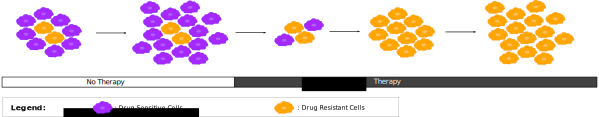
\includegraphics[width=\textwidth]{compe_release}
  \caption{Illustration of competitive release under SOC}
  \label{comperelease}
\end{figure}

\section{Adaptive therapy}
When competitive release happens, one could try to combat the cells with another drug or therapy method. However, these cells could potentially be resistant to the new drug as well and developing new drugs is research intensive. It would therefore be preferable to avoid such competitive release in the first place.

Adaptive therapy (AT) is one such novel approach to therapy under development to avoid competitive release. In AT, the cytotoxic drug is administered at lower and fluctuating doses in which the drug is administered at some lower dose for some duration, which would be followed by a drug holiday \cite{Gatenby}. This doesn’t kill off all the sensitive cells, and allows some fraction of them to remain in the microenvironment to prevent the resistant cells from taking over; this function of the sensitive cell fraction is thought to be due to the pressure of ecological competition they impose on resistant cells by competing with them for space and resources like oxygen. This competitive inhibition of resistant cells by the sensitive ones occurs during the drug holiday, when sensitive cells are not growth-limited by the drug. The tumour burden could then be kept under control as subsequent drug doses counteract the regrowth of sensitive cells during the drug holiday, as illustrated in \autoref{at}. The dosing schedule is therefore a central aspect of AT and must be designed to preserve the competitive inhibition of drug-resistant cells. One of the many regimes envisioned so far in the field uses tumour size as a metric to decide the timing of the dose and when the drug is withdrawn. The challenge with designing AT regimens is to balance the inhibition of resistant phenotype against absolute reduction of the overall tumour size. Adaptive therapy can be influenced by a wide range of factors that affect the dynamics and functioning of the system, and many of these parameters are under active investigation, including but not limited to cell turnover,  phenotypic heterogeneity, spatial constraints and fitness cost for resistance \cite{Strobl,Gallaher,Viossat,Bacevic}.

The promise of tumour control notwithstanding, it is worth noting that AT may not be able to achieve control indefinitely. It only attempts to improve the survival time and/or the time to relapse compared to other regimens and largely ignores the possibility of a cure, sometimes even where the standard of care method might yield better results. The patient has to live with the tumour for the rest of their life and other complications could arise due to this. Models are therefore being developed that could contribute to this decision-making process before therapy. The decision-making model would choose between the aggressive standard-of-care or adaptive therapy to either attempt cure or contain respectively after assessing the probability of cure as well as the risks and complications of maintaining a high tumour burden based on the composition of tumour \cite{Hansen}.

\begin{figure}[h]
  \centering
  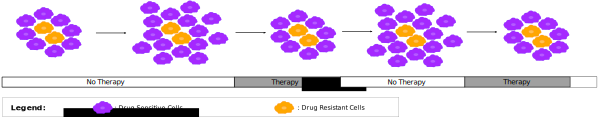
\includegraphics[width=\textwidth]{at}
  \caption{Illustration of control under AT}
  \label{at}
\end{figure}

\section{Importance of competition in adaptive therapy}
The only way of controlling the resistant phenotype for a fixed drug under AT is through competition by the sensitive cells. Therefore, the success of AT in containing the tumour depends on the effectiveness of competition between sensitive and resistant cells. It is frequently assumed that resistant cells are required to have an inherent growth disadvantage in the absence of the drug (cost of resistance) for AT to be successful, but it has been shown that the survival time can be prolonged by competition between the cells even without a cost of resistance \cite{Strobl}. Given that competition for resources between cell types can play such a central role in the success of AT regimens, a more detailed examination of how such competitive dynamics could play out would be a valuable addition to the existing literature. More specifically, a description of the competitive interactions between cancer cell types that is framed in terms of explicit resource dynamics along with cell population dynamics is a significant gap worth addressing.

\section{System of Study}
The metastatic castration resistant prostate cancer (mCRPC) was chosen to be the system of study. The mCRPC system already has a history of AT work done on it, although in different contexts \cite{Cunningham,Zhang}.

Prostate cells express androgen receptors (ARs) that require testosterone or its metabolite, 5-dihydrotestosterone to activate. Activated ARs bind to promoters of genes responsible for proliferation \cite{Heinlein}. Without testosterone, proliferation is halted and the cells die of apoptosis. When cancerous cells evolve from prostate cells, the AR mechanism is preserved and the cancer remains testosterone-dependent. However, mutant clones in prostate cancer occur that acquire mutations that allow them to synthesise their own testosterone independent of systemic supply, and these mutant clones are therefore the basis for acquisition of resistance to all forms of castration. Other mutations have also been shown in cancer cells to become entirely testosterone-independent, by acquiring mutations in the AR that make them constitutively active independent of testosterone.

This system is therefore usually modelled as consisting of three different types of cells: $T^+$, $T^p$ and $T^-$. $T^+$ is the baseline population for prostate cancer which requires testosterone for survival and is dependent on systemic supply of the hormone, with no internal sources. The standard therapy for prostate cancer is castration or androgen deprivation therapy (ADT) which blocks external production of testosterone and would kill the $T^+$ cells in a normal castration-sensitive prostate cancer. Castration-resistant prostate cancer cells are modelled as $T^p$ cells that can produce testosterone and sustain the $T^+$ cells. $T^p$ cells are also dependent on testosterone, and they synthesise testosterone from cholesterol through upregulation of the enzyme, CYP17$\alpha$ \cite{Dillard}. Finally, the hormone-independent non-producing fraction of the tumour is modelled as the $T^-$ cells, which do not require testosterone for cell growth. Abiraterone is a drug developed to specifically target castration resistance in prostate cancer that inhibits the CYP17$\alpha$ enzyme and can be effective against both $T^+$ and $T^p$, but would have no effect on $T^-$, as expected based on the functional differences between the three cell types.

\section{Goals of the Project}
This project has the following objectives in the context of adaptive therapy in the castration-resistant prostate cancer system.
\begin{enumerate}
  \item A model must be built of castration-resistant prostate cancer that includes explicit formal descriptions of resource dynamics alongside the dynamics of the three cell types detailed above. The rationale for this is to allow competition in the model to operate through the concentrations of the various resources that constitute the environment. This eliminates the need to estimate values of Lotka-Volterra type competition coefficients that are otherwise difficult to define and interpret based on clinical data.
  \item The model has three cell types which can be studied in stages, starting with two pairs: $T^p-T^-$ and $T^p-T^+$. The third pair, $T^+-T^-$ is a trivial case as $T^+$, with no internal or external sources of testosterone, would go extinct with or without $T^-$. The reason for starting with the pairwise interactions is to come up with a set of simpler observations about how resource concentrations affect competition between two cell types. These simpler observations can then be used to organise and interpret the outcomes of the full three-way competition between $T^p$, $T^+$ and $T^-$. Such a stepwise approach gives us a way to reduce the complexity of a system with three cell types and multiple resources, with each resource produced and consumed differently across the cell types.
  \begin{enumerate}
    \item While the differences of production and consumption of each resource between each cell type is the qualitative basis for interactions between them, these differences do not necessarily constitute competitive strategies, as the status of each cell type with respect to how it interacts with each resource is fixed. For example, if $T^p$ is dependent on testosterone for growth, the magnitude of its sensitivity to a low concentration of testosterone in the environment is the basis of its competitive strategy. While $T^p$ cannot become fully independent of testosterone, the minimum concentration of the hormone required for $T^p$ can be moved around to produce different strengths of competition for the hormone with $T^+$. Strategies of competition are therefore based on the extent to which a given cell type is limited by a resource, given that its mode of dependence is already defined.
    \item Given this definition of competitive strategies, the model can be used to explore competition in two separate contexts, depending on whether all three cell types have the same competitive strategy or each cell type is adopting a strategy unique to that type. Specifically, this is encoded in terms of the level of limitation of a given resource for each cell type. Additionally, both the initial population size and the relative proportion of each cell type in the initial tumour population would have significant effects on the outcomes of competition. Each of these strategies would therefore be studied across a range of population sizes and seeding ratios.
    \item Based on the previous two points, a comprehensive picture of competitive dynamics in the system can be assembled, with an understanding of how this picture is constructed based on the availability and utilisation of various resources.
  \end{enumerate}
  \item The application of therapy affects the ecological balance of this system in very specific ways, and the understanding of competitive interactions in the system based on resource dynamics also allows for outcomes of therapy to be explained in terms of how it affects competition.
  \begin{enumerate}
    \item Standard-of-care (SOC) treatment is the baseline approach against which adaptive therapy (AT) is to be evaluated. SOC involves constant application of the drug at the maximum tolerated dose (MTD). AT design includes at least two parameters-the threshold population sizes at which therapy must be turned on and off, and the gap between these two thresholds. Together, they form the therapy window within which the tumour must be contained. This window can be placed at a large or small population size, and can be wide or narrow. This would form the basis for the standardisation of the AT regimen used for the rest of the model.
    \item Once a standard AT regime is found, it would be applied to the model with all three cell types. As with the study of competition, the standardised AT regimen will be applied to all strategy conditions, across a range of population sizes and seeding densities.
  \end{enumerate}
\end{enumerate}
